\documentclass[a4paper,11pt]{article}

\usepackage{fullpage}
\usepackage{color}
\usepackage{hyperref}
\usepackage{amsmath}
\usepackage{amssymb}
\usepackage{tikz}
\usepackage{tabularx}
\usepackage{booktabs}
\usepackage{amsmath}
\usepackage{multirow}
\usepackage{layouts}
\usepackage{array}
\usepackage{pgf}
\usepackage{tikz}

\usepackage{amssymb}
\usepackage{graphics}
\usepackage{fancyhdr}
\usepackage{eucal}
\usepackage{ifthen}
\usepackage{ifpdf}
\usepackage{lmodern}
\usepackage{amsthm}
\usepackage{catoptions} % For \Autoref


\usetikzlibrary{positioning}

\hypersetup{
  colorlinks,%
    citecolor=black,%
    filecolor=black,%
    linkcolor=black,%
    urlcolor=mygreylink     % can put red here to visualize the links
}

\newcommand{\Pred}[2]{\ensuremath{\mathtt{Predator}\left<#1, #2\right>}}
\newcommand{\Prey}[2]{\ensuremath{\mathtt{Prey}\left<#1, #2\right>}}
\newcommand{\p}[2]{\ensuremath{\mathtt{P_{11^2}}\left<#1, #2\right>}}
\newcommand{\pSW}[2]{\ensuremath{\mathtt{P_{6^2}}\left<#1, #2\right>}}
\newcommand{\pRSW}[2]{\ensuremath{\mathtt{P_{6^2}}\left<#1, #2\right>}}
\newcommand{\SN}[0]{\ensuremath{S_{11^4}}}
\newcommand{\SSW}[0]{\ensuremath{S_{6^2}}}
\newcommand{\SRSW}[0]{\ensuremath{S_{21}}}

\newcommand{\rightuparrow}{\ensuremath{\rightarrow\!\!\!\!\!\uparrow}}
\newcommand{\rightdownarrow}{\ensuremath{\rightarrow\!\!\!\!\!\downarrow}}
\newcommand{\leftuparrow}{\ensuremath{\leftarrow\!\!\!\!\uparrow}}
\newcommand{\leftdownarrow}{\ensuremath{\leftarrow\!\!\!\!\downarrow}}

\newcommand{\DrawSmallPred}[2]{\node at (A.center #1 #2) {$\pi$};}
\newcommand{\DrawSmallPrey}[2]{\node at (A.center #1 #2) {P};}
\newcommand{\DrawBigPred}[2]  {\node at (A.center #1 #2) {\Huge $\pi$};}
\newcommand{\DrawBigPrey}[2]  {\node at (A.center #1 #2) {\Huge P};}


\newcommand{\resheading}[1]{{\large \colorbox{mygrey}{\begin{minipage}{\textwidth}{\textbf{#1 \vphantom{p\^{E}}}}\end{minipage}}}}

\newcommand{\mywebheader}{
  \begin{tabular}{@{}p{5in}p{4in}}
  {\resheading{Assignment 1: Single Agent Planning}} & {\Large 21 September, 2012}\\\vspace{0.2cm}
  \end{tabular}}

\begin{document}


\begin{center}
{\LARGE \textbf{Autonomous Agents}}\\ [1em] \vspace{0.1cm}
\Large\textbf{5 October 2012 }\\ \vspace{0.1cm}
\Large\text{Assignment 2: Single Agent Learning}
\end{center}


\begin{center}
{\Large By:} \\ \vspace{0.1cm}
{\Large Paris Mavromoustakos} \\  \vspace{0.1cm}
{\Large Georgios Methenitis} \\ \vspace{0.1cm}
{\Large Patrick de Kok} \\ \vspace{0.1cm}
{\Large Marios Tzakris}


\end{center}




\section*{Introduction}

In this assignment, we implement the learning scenario: the transition function is unknown to the agents, and so is the reward structure. We introduce model-based algorithms, which give agents the ability to learn high-reward policies while ignoring the model.  \\
Our code is based on the previous assignment, on which we added the classes necsessary to implement learning algorithms. Moreover, we have explicitly used the 21 statespace environment representation which reduced our algorithms' runtime on the previous assignment.


\section*{Exercise 1}

In this first exercise, we have implemented the Q-Learning algorithm with $\epsilon$-greedy action selection, as described  in chapter 6.5 of the Sutton and Barto book.\\
On each step of this algorithm, we chose an action $a$ of state $s$, and observed the next state and reward we got from it. Then, we updated the Q-learning table according to the following update rule: \\ 

$Q(s,a) \leftarrow  Q(s,a) + \alpha \left[ r + \gamma  max_{a'} Q(s',a') - Q(s,a)\right]$ \\

In this update rule, $Q(s,a)$ represents the value of the Q-learning table based on the previous step, while $Q(s',a')$ represents the observed state and possible actions, after action a is chosen. $Q(s,a)$ could be written as $Q(s_t,a_t)$ and $Q(s',a')$ as $Q(s_{t+1}, a_{t+1})$.\\
$\alpha$ represents the algorithm's learning rate, whereas $\alpha =0$ means that the Q-learning table will not be updated (the agent is not learning anything at all), while $\alpha =1$ means that that the agent learns based only on its immediate past.\\
$\gamma$ represents the discount factor, in the same way as described in DP algorithms, and $max_{a'}$ represents the action which is most likely to return the maximum reward among all the possible actions in state $s'$.

$\epsilon$ was given the value of 0.1 and the Q-learning table was initialized with 15.0 being assigned to all values. 


The figures below indicate the performance of the predator over time, given different values for $\alpha$ , and different values for $\gamma$.


\begin{figure} [ph]
\centering
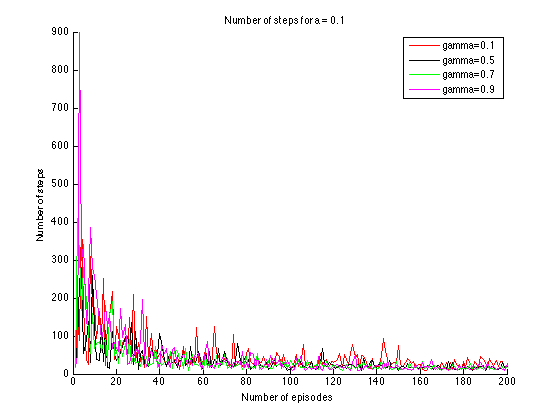
\includegraphics[width=1.0\textwidth,height=0.4\textheight]{a1.png}
\caption{Performance of Q-Learning with $\epsilon$-greedy for $\alpha = 0.1$.}
\label{Figure 1}
\end{figure}

\begin{figure} [H!]
\centering
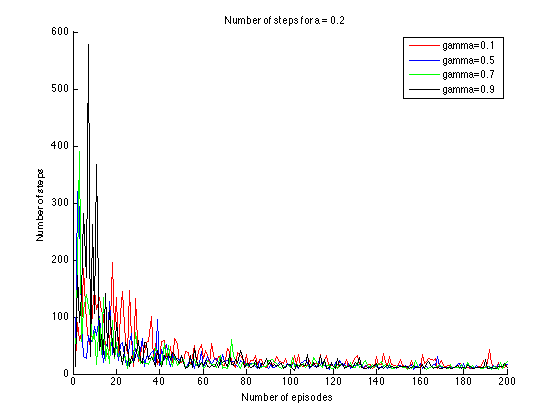
\includegraphics[width=1.0\textwidth,height=0.4\textheight]{a2.png}
\caption{Performance of Q-Learning with $\epsilon$-greedy for $\alpha = 0.2$.}
\label{Figure 2}
\end{figure}


\begin{figure} [H!]
\centering
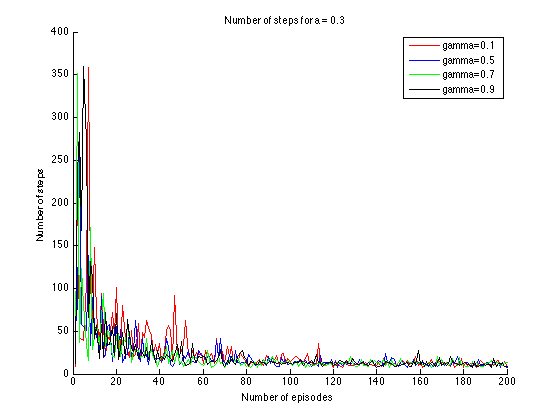
\includegraphics[width=1.0\textwidth,height=0.4\textheight]{a3.png}
\caption{Performance of Q-Learning with $\epsilon$-greedy for $\alpha = 0.3$.}
\label{Figure 3}
\end{figure}

\begin{figure} [H!]
\centering
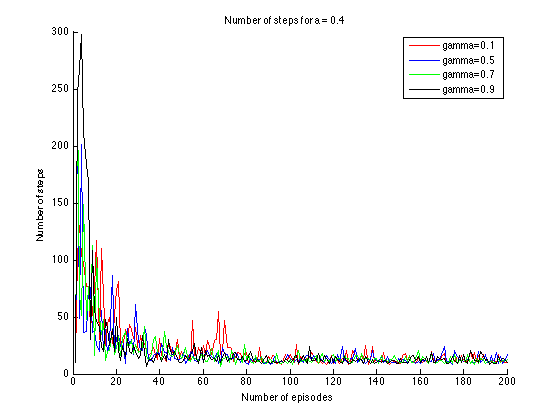
\includegraphics[width=1.0\textwidth,height=0.4\textheight]{a4.png}
\caption{Performance of Q-Learning with $\epsilon$-greedy for $\alpha = 0.4$.}
\label{Figure 4}
\end{figure}

\begin{figure} [h!]
\centering
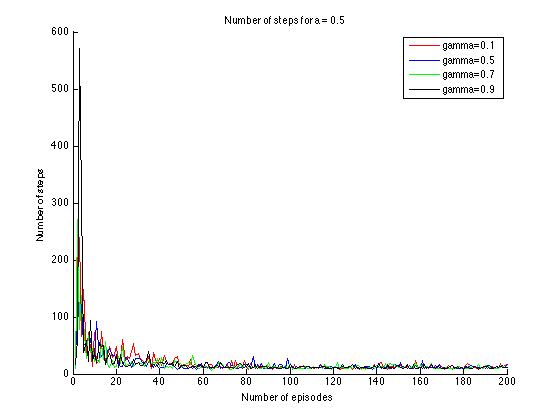
\includegraphics[width=1.0\textwidth,height=0.4\textheight]{a5.png}
\caption{Performance of Q-Learning with $\epsilon$-greedy for $\alpha = 0.5$.}
\label{Figure 5}
\end{figure}


The graphs 1-5 clearly indicate how the predator learns faster while we increment the value of $\alpha$. Figure 1 shows us that for $\alpha = 0.1$ the predator needs about 150 episodes to converge to the optimal policy. However, while we increase alpha, the predator will need less episodes for its Q-learning table to converge. \\
Increasing the value of $\alpha$ means that we consider the most recent information we observe, more important. A value of $\alpha = 0$ would mean that the predator is not learning at all, while $\alpha = 1$ means that the predator only obtains information from its immediately previous actions. 
 
\section*{Exercise 2}

In this exercise we have implemented Q-learning with $\epsilon$ -greedy action decision for different values for $\epsilon$ , using different initial values for the Q-learning table each time. We have used 3 different values for the initialization of the Q-table, a pessimistic one (5), a realistic one (10) and an optimistic one (15), to see how the agent behaves for different values of $\epsilon$ in each case.

We have chosen particular values for $\epsilon$ to test how, and what the predator learn to do. For $\epsilon = 0$, the predator will always choose the action for which the Q-learning table has maximum value, thus, the agent will converge to the optimal path really fast if the initial values of the Q-table are lower than the immediate reward of the absorbing state, but it will become explorative if the Q-table values are optimistically initialized.


If $\epsilon = 0.1$, the agent will try to exploit the action for which the Q-table has the maximum value with a probability of $1-\epsilon = 0.9$. That means that our predator is trying to exploit more than it is trying to explore, and there is a small probability that it will not choose the action it considers optimal.

We have used the value of 0.8 for $\epsilon$ aswell, because in this case, each possible action for the predator might have the same probability to be chosen. For example, if the predator has 5 possible actions, there will be $1-\epsilon = 0.2$ probability for the "optimal" action to be chosen, and each of the other possible states will also have $\epsilon /4 = 0.2$ probability to be chosen. As a consequence, in the best case scenario our agent will be moving randomly. If there are less than 5 possible moves, he will be most likely be choosing one of the "non-optimal" moves.

Finally, we have also included $\epsilon = 0.99$ in our experimentation, for the reason that this value leaves almost zero probability for the agent to choose the optimal action. So, what happens in this case is that the predator learns not to use the optimal action each time he has to take a decision, so as we see in the graphs, the number of steps it takes him to find the prey is increased dramatically as time goes by.

\section*{Exercise 3}

\section*{Exercise 4}


\section*{Exercise 5}


\section*{Conclusion}

\end{document}
